\documentclass{article}
%=============================================================================80
%	                          Packages                                     %
%==============================================================================%
% Packages
\usepackage[utf8]{inputenc}
\usepackage{graphicx}
\usepackage{amsmath}
\usepackage{mathtools}
\usepackage{amssymb}
\usepackage{braket}
\usepackage{float}
\usepackage{hyperref}
\usepackage{subcaption}
\usepackage[margin=0.7in]{geometry}
\usepackage[version=4]{mhchem}
\usepackage{cite}
%==============================================================================%
%                           User-Defined Commands                              %
%==============================================================================%
% User-Defined Commands
\newcommand{\be}{\begin{equation}}
\newcommand{\ee}{\end{equation}}
\newcommand{\benum}{\begin{enumerate}}
\newcommand{\eenum}{\end{enumerate}}
\newcommand{\pd}{\partial}
\newcommand{\dg}{\dagger}

%==============================================================================%
%                             Title Information                                %
%==============================================================================%
\title{PIMD Notes}
\date{11/14/19}
\author{Alan Robledo}
%==============================================================================%
\begin{document}

\maketitle

I have created the following notes to better understand path integral molecular dynamics (PIMD) as applied to a harmonic oscillator and beyond. All the material in this paper can be found in mutliple resources. The ones that I used are listed in the references. Notes are still in development.

\section{Introduction}
\subsection{Quantum Harmonic Oscillator}
Similar to the classical harmonic oscillator, we have a particle that is subject to a harmonic potential so that the 1D Hamiltonian looks like
\be \label{eq:harm_osc}
  \hat{H} = \hat{K} + \hat{U} = \frac{\hat{p}^2}{2m} + \frac{1}{2}m \omega^2\hat{x}^2
\ee
where $m$ is the particle's mass and $\omega$ is the angular frequency of the oscillator.
We know that we can derive the properties of the harmonic oscillator from the canonical ensemble. To do this, we start with the canonical partition function,
\be \label{eq:classical_part_func}
  Q = \sum_n e^{-\beta E_n}
\ee
where the sum is performed over all possible states of the system, which are discrete.\cite{tuckerman}
The energies $E_n$ for a quantum harmonic oscillator are well known and can be obtained from solving Schr\"odinger's equation with the Hamiltonian in equation (\ref{eq:harm_osc}).
Alternatively, the energies can be derived (see Appendix 1) using Dirac's ladder operators, $\hat{a}$ and $\hat{a}^{\dagger}$.\cite{griffiths,shankar}
Doing so yields,
\be
  E_n = \hbar \omega(n + \frac{1}{2}) .
\ee
Plugging our energies into equation (\ref{eq:classical_part_func}) gives us the partition function.
\be \label{eq:harm_part_func}
  Q = \sum_{n=0}^{\infty} e^{-\beta \hbar \omega(n + \frac{1}{2})}
\ee

The purpose of knowing the partition function is so that we can derive the thermodynamic properties of our system in the canonical ensemble. One property we can derive is the total energy. We already know the energies of the harmonic oscillator, but we can derive the energies in the canonical ensemble with the partition function using the relationship,
\be
  E = - \frac{\partial}{\partial \beta} \ln(Q) .
\ee
Using equation (\ref{eq:harm_part_func}), we find (see Appendix 2) that the energies are of the form,
\be \label{eq:canonical_energies}
  E = \frac{\hbar \omega}{2} + \frac{\hbar \omega e^{-\beta \hbar \omega}}{1-e^{-\beta \hbar \omega}}.
\ee

Remember that this is the exact form of the harmonic oscillator energies in the canonical ensemble and not an approximation. When we try to approximate the energies of a harmonic oscillator using PIMD, we will want to refer back to equation (\ref{eq:harm_canonical_e}) and plug in our values for $\omega$ and $\beta$ as a check to make sure that our code is working.

To understand what a PIMD code does, we have to first understand the idea of representing partition functions like equation (\ref{eq:harm_part_func}) as a path integral.

\subsection{Path Integral Representation}
We will consider the case of a single quantum particle moving in one dimension subject to some potential $U(x)$.
Remember that our Hamiltonian is, in general,
\be
  \hat{H} = \hat{K} + \hat{U} .
\ee
We already know from classical statistical mechanics that the canonical partition function can be written as equation (\ref{eq:harm_part_func}).
In Quantum Statistical Mechanics, the parition function is written more formally as (see Appendix 3),
\be \label{eq:quan_part_func}
  Q(N, V, T) = \text{Tr}\Big[ e^{- \beta \hat{H}} \Big]
\ee
where $\beta = 1/k_BT$ and $\hat{H}$ is the Hamiltonian of our system.

If we perform the trace in the coordinate basis, we obtain an integral
\be \label{eq:part_func_coord}
  Q = \text{Tr} \Big[e^{-\beta \hat{H}}\Big] = \int dx \braket{x|e^{-\beta \hat{H}}|x} .
\ee
After going through a long process (see Appendix 4), equation (\ref{eq:part_func_coord}) can be represented equaivalently in terms of path integrals,
% Might use bottom later
%===========================================================================%
% The amplitude of a path that the particle can take when going from x to x' over some time t as the propagator written in position space.
% \be
%   A = \braket{x'|e^{-iHt/\hbar}|x}
% \ee
% This is useful to know because the probability of the particle choosing a particular path would simply be $|A|^2$.\cite{tuckerman}
% In terms of state vectors, the initial state of our particle can be represented as $\ket{\Psi(0)}$, so the state of our particle can be represented as the inital state vector being acted upon by the propagator
% \be
%   \ket{\Psi(t)} = e^{-iHt/\hbar} \ket{\Psi(0)}
% \ee
% And we can project the coordinate basis onto our state vectors to give us a meaningful representation of our state vector
% \be
%   \begin{split}
%     \braket{x'|\Psi(t)} = \Psi(x',t) &= \braket{x'|e^{-iHt/\hbar}|\Psi(0)} \\
%     &= \braket{x'|e^{-iHt/\hbar}\int dx|x} \braket{x|\Psi(0)} \\
%     &= \int dx \braket{x'|e^{-iHt/\hbar}|x} \braket{x|\Psi(0)} \\
%     &= \int dx \braket{x'|e^{-iHt/\hbar}|x} \Psi(x,0)
%   \end{split}
% \ee
% where we introduced the resolution of identity $\int dx \ket{x} \bra{x} = 1$.
%
% So now we have a more mathematical representation of our problem; we want to know how to go from $\Psi(x,0)$ to $\Psi(x',t)$.
% The physical representation of our problem is that we have a particle at some point x in space, and we want to be able to detect our particle at some other point x' in space after some time t passes.
%
% By going to imaginary time, which is done by substituting $it/\hbar = \beta$, we can express the coordinate-space quantum propagator as the canonical density matrix,
% \be \label{eq:density_mat}
%   \rho(x,x') = \braket{x'|e^{-\beta \hat{H}}| x} .
% \ee
% The motive behind doing this is so that we can deal with a damped exponential as opposed to a complex exponential.\cite{tuckerman}
% Therefore, we can derive the path integral form of the density matrix and simply resubstitute time in place of $\beta$ to obtain the path integral form of the time propagator.
%===========================================================================%
\be \label{eq:pimd_partition}
  Q = \lim_{P \to\infty} \int dp_1 \cdots dp_P \int dx_P \cdots dx_1 \quad \text{exp}\Big( - \beta \sum_{k=1}^P \Big[ \frac{p^2_k}{2m'} + \frac{1}{2} m \omega^2_P (x_{k+1} - x_k)^2 + \frac{1}{P} U(x_k) \Big] \Big) .
\ee
The interesting thing about the path integral representation is that equation (\ref{eq:pimd_partition}) resembles the classical partition function for a cyclic chain of beads.
Each bead can be thought of as having the same fictious mass m' along with harmonic nearest neighbors.
In other words, each bead is connected to one another with a spring that is defined by the chain frequency $\omega_P = \sqrt{P}/(\beta \hbar)$.
Lastly, each bead is subjected to an external potential $U(x)$ that is defined by the quantum system.

Therefore, the properties of our quantum system can be obtained directly from the classical system in the infinite bead limit.
Alternatively, these quantities can be approximated by performing calculations with a finite number of beads and is the main idea behind a PIMD calculation.
It is worth mentioning that quantum properties of interest can also be uncovered by decreasing the temperature of our system or the masses of our beads.

Going back to the 1D quantum harmonic oscillator, a PIMD calculation would consist of performing a moecular dynamics simulation on one chain of P beads with each bead subject to an external potential $U(x) = (1/2)m \omega^2 x^2$, which defines the quantum oscillator.
The temperature of our system can be controlled by introducing a thermostat.
Thermostats also allow us to make sure that we are sampling the canonical distribution when running a molecular dynamics code.

\subsection{Path Integral Molecular Dynamics}
Mapping a quantum system of interest onto a classical system of cyclic chains allows us to use a molecular dynamics scheme on a Hamiltonian of the form
,
\be \label{eq:chain_hamiltonian}
  H = \Big[ \frac{p^2_k}{2m'} + \frac{1}{2} m \omega^2_P (x_{k+1} - x_k)^2 + \frac{1}{P} U(x_k) \Big] .
\ee
A more feasible way to perform an MD calculation on a coupled system is to introduce a coordinate transformation that de-couples each degree of freedom.
The harmonic coupling term in equation (\ref{eq:chain_hamiltonian}) can become uncoupled by introducing staging coordinates.\cite{tuckerman}
A staging coordinate transformation converts the original set of coordinates, which we refer to as primitive coordinates, $\{x_1 , x_2 , \dots , x_P \}$ into a set of staging coordinates $\{u_1 , u_2 , \dots , u_P \}$.
In one dimension, each staging coordinate is defined as,
\be
  \begin{split}
    u_1 &= x_1 \\
    u_k &= x_k - \frac{(k-1)x_{k+1} + x_1}{k} \quad \quad k = 2, \dots, P\\
  \end{split}
\ee
The Hamiltonian in staging coordinates becomes,
\be
  H = \Big[ \frac{p^2_k}{2m'_k} + \frac{1}{2} m_k \omega^2_P u_k^2 + \frac{1}{P} U(x_k(u)) \Big] .
\ee
where a set of fictitious masses $m_k$ are defined as,
\be
  \begin{split}
    m_1 &= 0 \\
    m_k &= \frac{k}{k-1} m \quad \quad k = 2, \dots, P
  \end{split}
\ee
and $m'_k$ are defined as,
\be
  \begin{split}
    m'_1 &= m \\
    m'_k &= m_k = \frac{k}{k-1} m \quad \quad k = 2, \dots, P .
  \end{split}
\ee
Since the potential $U(x_k(u)$ is defined as the potential from the original quantum system, a PIMD calculation requires performing an inverse staging coordinate transformation in order to compute the potential in the primitive coordinates.

A typical PIMD simulation then makes use of the equations of motion defined in staging coordinates,
\be
  \begin{split}
    \dot{u}_k &= \frac{p_k}{m'_k} \\
    \dot{p}_k &= - m_k \omega_P^2 u_k - \frac{1}{P} \frac{\partial U}{\partial u_k} \\
  \end{split}
\ee
where the forces on the staging coordinates $- \frac{\partial U}{\partial u_k}$ are defined recursively as,
\be
  \begin{split}
    \frac{1}{P} \frac{\partial U}{\partial u_1} &= \frac{1}{P} \sum_{l-1}^{P} \frac{\partial U}{\partial x_l} \\
    \frac{1}{P} \frac{\partial U}{\partial u_k} &= \frac{1}{P} \Big[ \frac{\partial U}{\partial x_k} + \frac{k-2}{k-1} \frac{\partial U}{\partial u_{k-1}}\Big] \quad \quad k = 2,\dots, P .
  \end{split}
\ee
The thermostat is then implemented to ensure proper sampling of the canonical ensemble.\cite{Liu}

When performing a PIMD calculation, thermodynamic estimators are often used to approximate values of thermodynamic quantities.
The virial energy estimator is what we will focus on for testing a PIMD code.
The virial energy,
\be
  E_vir = \frac{1}{P} \sum_{k=1}^P \Big[ \frac{1}{2}x_k \frac{\partial U}{\partial x_k} + U(x_k) \Big]
\ee
can be computed at every step of a simulation to obtain a plot of instantaneous virial energies and cumulative averages.
The thermal coupling will cause the instantaneous virial energies to fluctuate, but the cumulative averages should stay consistent after the system begins to equilibrate.
For a quantum harmonic oscillator, we can expect the virial energy to approximate the energies in the canonical ensemble (equation \ref{eq:canonical_energies}).

\section{Results}
Since the PIMD code that I have written consists of combining velocity verlet with a langevin thermostat, several test cases were done to check that each piece was implemented properly.

\subsection{Velocity Verlet}
The first test case was writing a velocity verlet code for a one dimensional harmonic oscillator.
The dynamics for these simulations were entirely deterministic due to the lack of any thermostat coupling.
Therefore, replicating key features of the classical harmonic oscillator became the goal to verify that the code was written well.

\begin{figure}[H]
  \centering
  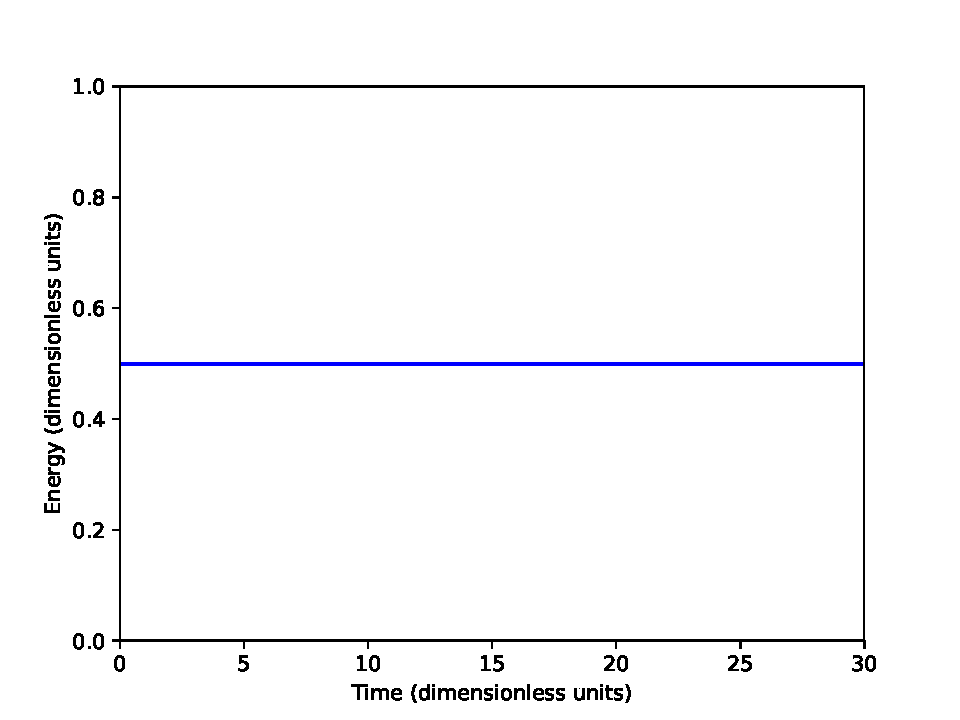
\includegraphics[scale=0.7]{Figures/1dverlet/energies.pdf}
    \caption{Plot of total energy for a harmonic oscillator ($m = \omega = 1$) over an MD trajectory. The energy remains constant throughout an MD trajectory because there are no other external forces acting on the potential, which conserves total energy. Initial conditions for the simulation was: $x(0) = 0, v(0) = 1$. Plugging these values along with the mass and frequency into the Hamiltonian shows that the energy should be 0.5 throughout the trajectory.}
\end{figure}

Since there is no energy exhange occuring throughout a simulation, the energy of the oscillator should remain constant throughout a trajectory. The exact value of the energy at each time step will vary by some amount depending on the precision of each calculation, but a plot of the energy over time should yield a horizontal line (Figure 1).

Solving newton's equations for a harmonic oscillator yields,
\be
  x(t) = A \cos(\omega t + \phi)
\ee
where $\omega$ is the frequency of the oscillator.
Therefore, plotting the position of an oscillator with a small frequency should result in a wave with a large wave period.
In contrast, plotting the position of an oscillator with a large frequency should result in a wave with a small wave period (Figure 2).
\begin{figure}[H]
    \centering
    \begin{subfigure}[b]{0.49\textwidth}
        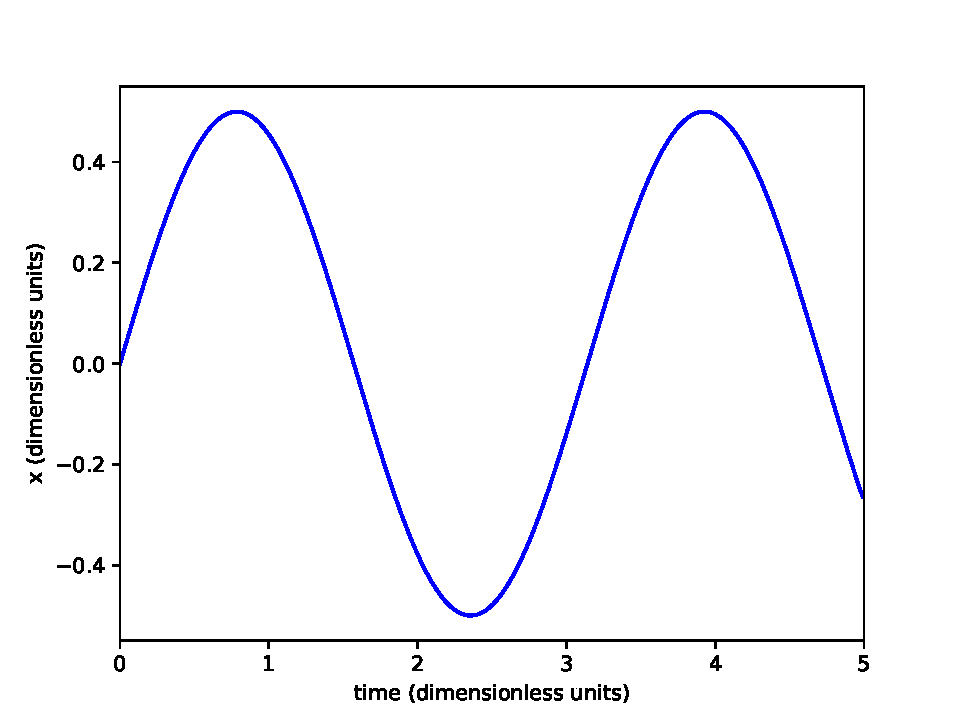
\includegraphics[width=\textwidth]{Figures/1dverlet/positw2.pdf}
  	\caption{Positions with $\omega = 2$.}
    \end{subfigure}
    \begin{subfigure}[b]{0.49\textwidth}
        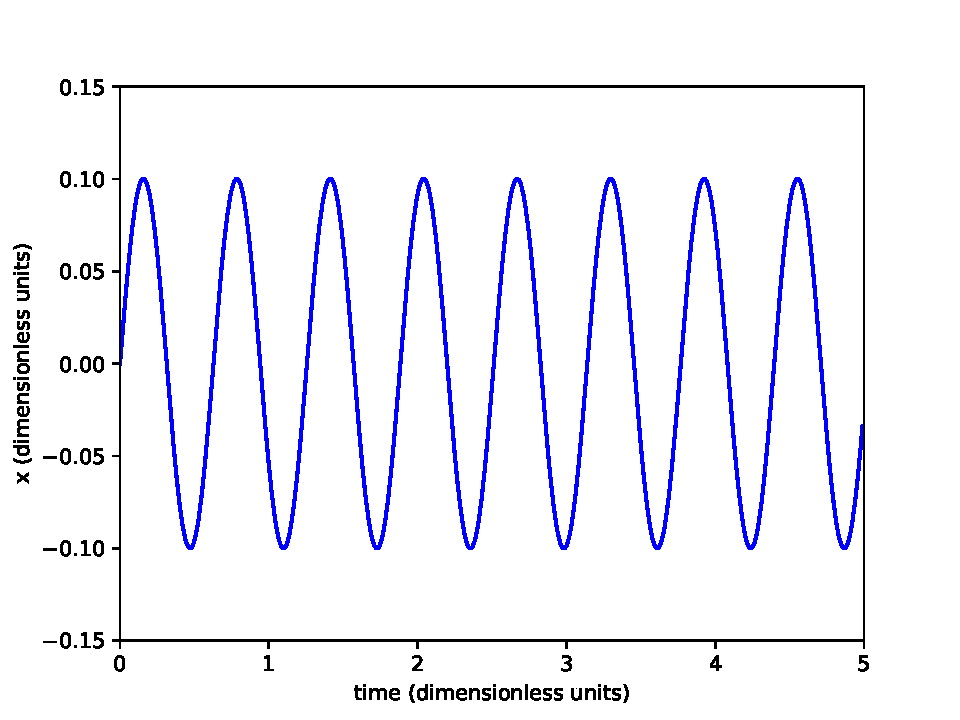
\includegraphics[width=\textwidth]{Figures/1dverlet/positw10.pdf}
        \caption{Positions with $\omega = 10$}
    \end{subfigure}
    \caption{Harmonic oscillator ($m = 1$) positions for different values of frequency $\omega$. Initial conditions for the simulations were: $x(0) = 0, v(0) = 1$.}
\end{figure}
The Hamiltonian for a harmonic oscillator tells us that a phase space plot should result in an ellipse (Figure 3).
Remembering that the equation for an ellipse centered at (0,0) is
\be
  1 = \frac{x^2}{a^2} + \frac{y^2}{b^2}
\ee
we can define the semi-major axis of the phase space plot as $a = \sqrt{\frac{2E}{m \omega^2}}$ and the semi-minor axis of the phase space plot as $b = \sqrt{2mE}$.
\begin{figure}[H]
  \centering
  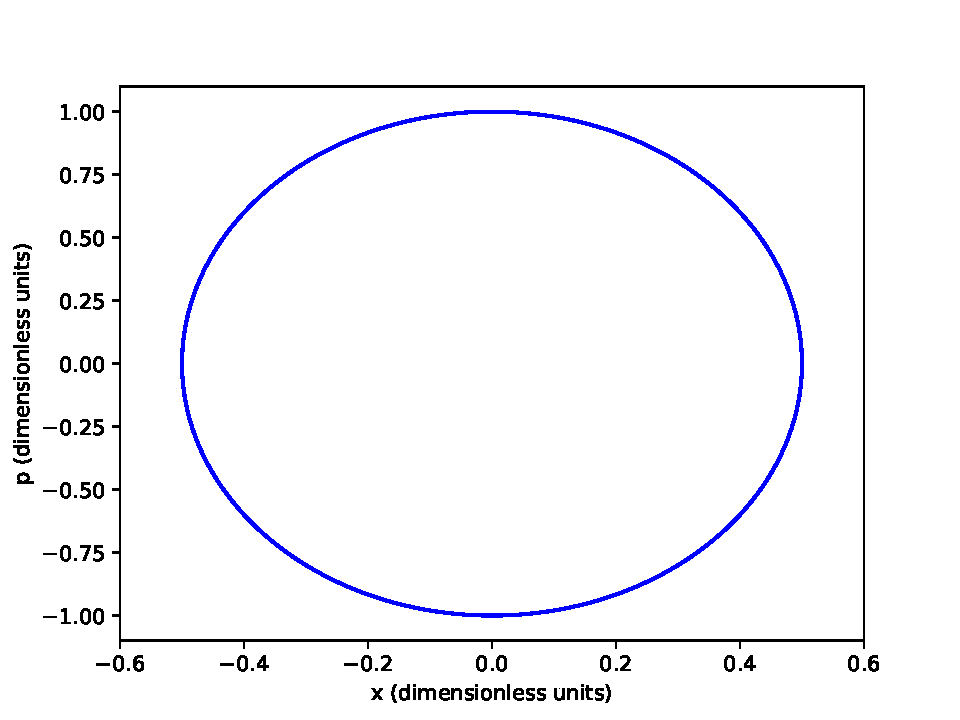
\includegraphics[scale=0.7]{Figures/1dverlet/phasespace_w2.pdf}
    \caption{Phase space plot of the one dimensional harmonic oscillator ($m = 1$) with $\omega = 2$. The phase space curve should follow the shape of an ellipse since the Hamiltonian is $H = \frac{1}{2m}p^2 + \frac{m \omega^2}{2}x^2$. Initial conditions for the simulations was: $x(0) = 0, v(0) = 1$.}
\end{figure}
An MD simulation of 3 coupled harmonic oscillators ($m_1 = m_2 = m_3 = m$ , $\omega_1 = \omega_2 = \omega_3 = \omega$) was done to test the verlet code with a different potential.
This system was non-periodic with fixed boundary conditions, i.e. mass 1 was connected to wall by a spring and mass 3 was connected another wall by another spring.
The Hamiltonian for this system is equal to
\be
  H = \sum_{i=1}^{3} \frac{p_i^2}{2 m} + m \omega^2 (x_{i+1} - x_{i})^2 .
\ee
The purpose of this test was to verify the positions of each mass during an MD simulation done by Gren and Wahnstr of the same system (Figure 4).
The initial conditions were such that mass 1 started at $x_1 = 0.1$ and mass 2 and 3 started at $x_2 = x_3 = 0$.
The plot in Figure 4 shows that mass 1 moves opposite of masses 2 and 3, which makes sense because the system is defined as mass 1 having some displacement to the left of mass 2.
Therefore, if mass 1 starts to the right of mass 2, the simulation should show mass 1 moving to the left and mass 2 moving to the right for some $\Delta t$.
\begin{figure}[H]
  \centering
  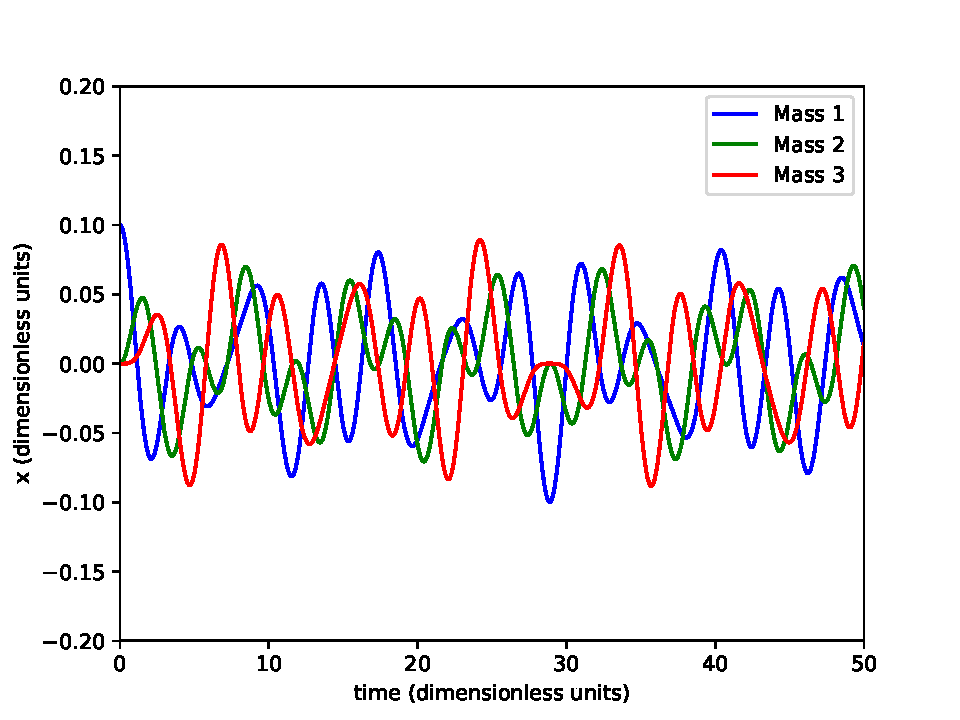
\includegraphics[scale=0.7]{Figures/1dverlet/3part_2walls.pdf}
    \caption{Plot of positions for each mass over time for 3 non-periodic coupled harmonic oscillators without thermostat coupling and with fixed boundary conditions. The purpose of this plot was to replicate the results of the same calculation done by Gren and Wahnstr\"om.\cite{gren}}
\end{figure}

\subsection{Langevin Dynamics with Velocity Verlet}
Another code was written for a classical one dimensional harmonic oscillator coupled to a langevin thermostat.
The langevin step added to the velocity verlet is done so that a random kick is added to the system at each time step that depends on a random variable sampled from the normal distribution with mean $\mu = 0$ and standard deviation $\sigma^2 = 1$.
For this reason, histograms of the positions and momenta for the oscillator should mimic a gaussian distribution (Figure 5).
\begin{figure}[H]
    \centering
    \begin{subfigure}[b]{0.49\textwidth}
        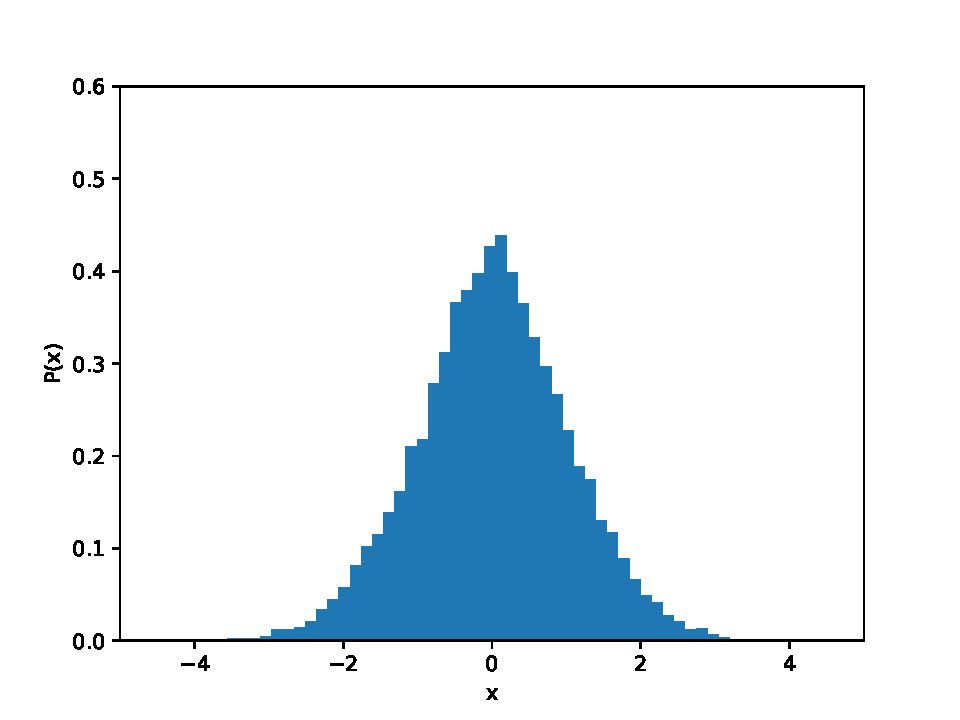
\includegraphics[width=\textwidth]{Figures/langevin/xhist.pdf}
    \end{subfigure}
    \begin{subfigure}[b]{0.49\textwidth}
        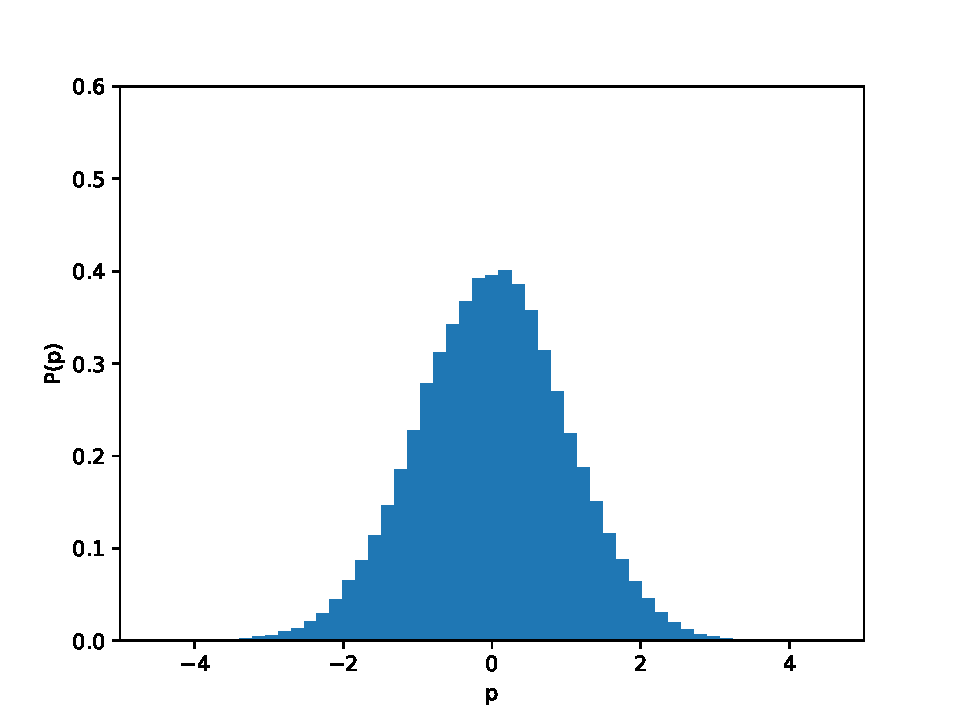
\includegraphics[width=\textwidth]{Figures/langevin/phist.pdf}
    \end{subfigure}
    \caption{Histograms of position (a) and momenta (b) for the one dimensional harmonic oscillator ($m = 1$). Initial conditions for the simulation was: $x(0) = 0, v(0) = 0.1$. The friction $\gamma = K_B T$ in this simulation. The choice for this value of the friction came from the optimum value of the friction coefficient being $\gamma = \omega_P$, as stated in the paper by Liu.\cite{Liu} In this case, P = 1.}
\end{figure}

\subsection{Path Integral Molecular Dynamics}
Finally, the PIMD code was written to replicate the results done by Tuckerman et al.\cite{tuckerman}
The system defined by Tuckerman et al consisted of a one dimensional quantum harmonic oscillator with $\beta \hbar \omega = 15.8$, $m \omega / \hbar = 0.03$, and $P = 400$.
These parameters are used so that the thermodynamic energy is dominated by the ground state energy.
Therefore, we expect a proper PIMD calculation to yield energies equal to $\hbar \omega / 2$ (Figure 6).

\begin{figure}[H]
  \centering
  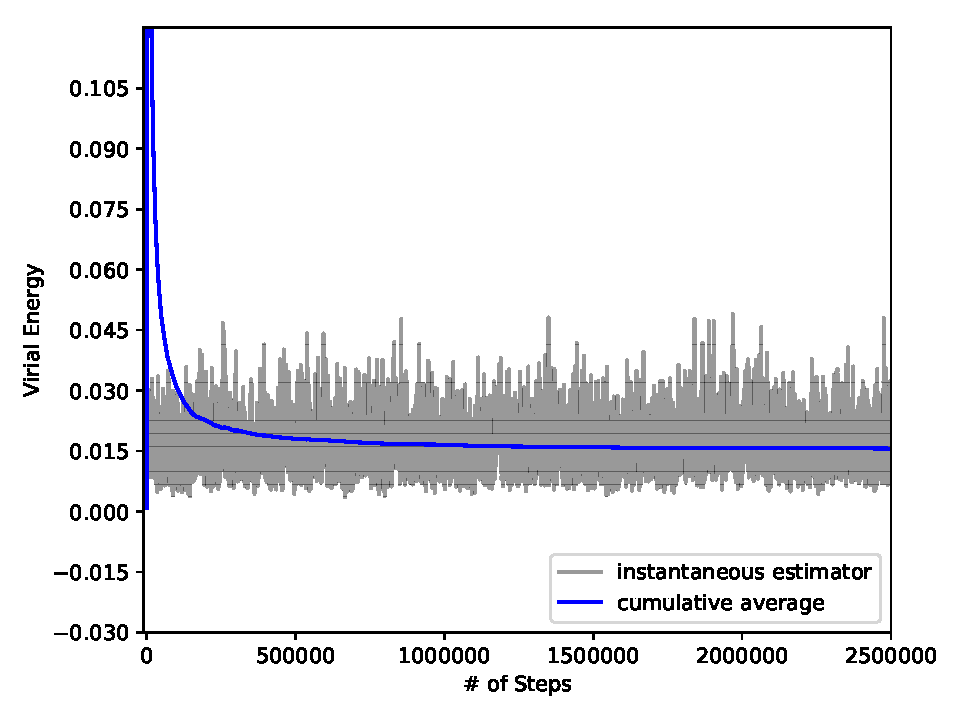
\includegraphics[scale=0.7]{Figures/pimd/smallkt.pdf}
    \caption{Plot of the instantaneous virial estimator along with cumulative averages along a PIMD trajectory. Since the simulation was performed in using atomic units, we defined variables $\hbar = m = K_B = 1$ so that $\omega = 0.03$ and $T = 0.03/15.8$. Simulations were considered successful if the cumulative average of the virial estimator converged at $E_vir = \hbar \omega / 2 = 0.015$. This simulation converged at a value of 0.0156 after 2,500,000 million MD steps with $\Delta t = 0.01$. Initial conditions for this simulation were $u_k(0) = 0$ and $v_k(0) = 1$.}
\end{figure}

\section{Appendix}
\subsection{Quantum Harmonic Oscillator Energies}
This section serves to derive the energies for a quantum harmonic oscillator using Dirac's ladder operators.

The "raising operator" $\hat{a}$ and "lowering operator" $\hat{a}^{\dagger}$ can be defined in terms of the position and momentum operators as
\be
  \begin{split}
    \hat{a} &= \sqrt{\frac{m \omega}{2 \hbar}} \Big( \hat{x} + \frac{i}{m \omega} \hat{p}\Big) \\
    \hat{a}^{\dagger} &= \sqrt{\frac{m \omega}{2 \hbar}} \Big( \hat{x} - \frac{i}{m \omega} \hat{p}\Big)
  \end{split}
\ee
where the prefactors are such that they allow the math to work out nicely when deriving the energies for a harmonic oscillator.
The ladder operators can then be used to obtain a function of the Hamiltonian by remembering the commutation relation $[\hat{x},\hat{p}] = i \hbar$. The hats will be ommited from the operators to simplify notation.
\be
  \begin{split}
    aa^{\dagger} &= \sqrt{\frac{m \omega}{2 \hbar}} \Big( x + \frac{i}{m \omega} p\Big) \sqrt{\frac{m \omega}{2 \hbar}} \Big( x - \frac{i}{m \omega} p\Big) \\
    &= \frac{m \omega}{2 \hbar} \Big( x + \frac{i}{m \omega} p\Big) \Big( x - \frac{i}{m \omega} p\Big) \\
    &= \frac{m \omega}{2 \hbar} \Big( x^2 - \frac{i}{m \omega}xp + \frac{i}{m \omega}px + \frac{p^2}{(m \omega)^2} \Big) \\
    &= \frac{m \omega}{2 \hbar} \Big( x^2 + \frac{p^2}{(m \omega)^2} \Big) - \frac{i}{2 \hbar}xp + \frac{i}{2 \hbar}px \\
  \end{split}
\ee
We can turn everything in the paranthesis into the Hamiltonian after mutliplying by $1=\frac{m \omega}{m \omega}$ and distributing the $\frac{1}{2}$.
\be
  \begin{split}
    aa^{\dagger} &= \frac{m \omega}{2 \hbar} \Big( \frac{m \omega}{m \omega} \Big) \Big( x^2 + \frac{p^2}{(m \omega)^2} \Big) - \frac{i}{2 \hbar}xp + \frac{i}{2 \hbar}px \\
    &= \frac{1}{2 \hbar} \Big( \frac{p^2}{m \omega} + m \omega x^2\Big) - \frac{i}{2 \hbar} [x,p] \\
    &= \frac{1}{\hbar \omega} \Big( \frac{p^2}{2m} + \frac{(m \omega x)^2}{2m}\Big) - \frac{i}{2 \hbar} (i \hbar) \\
    &= \frac{1}{\hbar \omega} H + \frac{1}{2}
  \end{split}
\ee
So rearranging to solve for the Hamiltonian gives us,
\be \label{eq:h_plusminus}
  \hat{H} = \hbar \omega \Big( \hat{a} \hat{a}^{\dagger} - \frac{1}{2} \Big) .
\ee
If we reverse the ladder operators and perform the same process as before we get,
\be
  \begin{split}
    a^{\dagger}a &= \sqrt{\frac{m \omega}{2 \hbar}} \Big( x - \frac{i}{m \omega} p\Big) \sqrt{\frac{m \omega}{2 \hbar}} \Big( x + \frac{i}{m \omega} p\Big) \\
    &= \frac{m \omega}{2 \hbar} \Big( x - \frac{i}{m \omega} p\Big) \Big( x + \frac{i}{m \omega} p\Big) \\
    &= \frac{m \omega}{2 \hbar} \Big( x^2 + \frac{i}{m \omega}xp - \frac{i}{m \omega}px + \frac{p^2}{(m \omega)^2}\Big) \\
    &= \frac{m \omega}{2 \hbar} \Big( x^2 + \frac{p^2}{(m \omega)^2}\Big) + \frac{i}{2 \hbar}xp - \frac{i}{2 \hbar}px \\
    &= \frac{m \omega}{2 \hbar} \Big( \frac{m \omega}{m \omega} \Big) \Big( x^2 + \frac{p^2}{(m \omega)^2}\Big) + \frac{i}{2 \hbar}xp - \frac{i}{2 \hbar}px \\
    &= \frac{1}{2 \hbar} \Big( \frac{p^2}{m \omega} + m \omega x^2 \Big) + \frac{i}{2 \hbar} [x,p] \\
    &= \frac{1}{2 \hbar m \omega} \Big( p^2 + (m \omega x)^2 \Big) + \frac{i}{2 \hbar} (i \hbar) \\
    &= \frac{1}{\hbar \omega} \Big( \frac{p^2}{2m} + \frac{(m \omega x)^2}{2m} \Big) - \frac{1}{2} \\
    &= \frac{1}{\hbar \omega}H - \frac{1}{2}
  \end{split}
\ee
So rearranging to solve for the Hamiltonian gives us,
\be \label{eq:h_minusplus}
  \hat{H} = \hbar \omega \Big(\hat{a}^{\dagger} \hat{a} + \frac{1}{2} \Big) .
\ee
We can imagine a set of vectors that make up the basis of eigenvectors $\ket{\psi_n}$ for the harmonic oscillator Hamiltonian that yield energies $E_n$.
If we apply equation (\ref{eq:h_plusminus}) to a vector that is one state higher $\hat{a}\ket{\psi_n}$, we obtain,
\be
  H \hat{a}\ket{\psi} = (E_n + \hbar \omega) \hat{a}\ket{\psi}.
\ee
eigenvalues equal to the energy in the previous state plus $\hbar \omega$.
Likewise, if we apply equation (\ref{eq:h_minusplus}) to a vector that is one state lower $\hat{a}^{\dagger}\ket{\psi_n}$, we obtain,
\be
  H \hat{a}^{\dagger}\ket{\psi} = (E_n - \hbar \omega) \hat{a}^{\dagger}\ket{\psi} .
\ee
It is for this reason that the operators $\hat{a}$ and $\hat{a}^{\dagger}$ are called ladder operators because they allow us to go up and down in energy.\cite{griffiths,shankar}
When we consider that there is a ground state $\ket{\psi_0}$ such that $\hat{a}^{\dagger}\ket{\psi_0} = 0$, we can plug in the defintion for $\hat{a}^{\dagger}$ in position space,
\be
  \hat{a}^{\dagger} \ket{\psi_0} = \sqrt{\frac{m \omega}{2\hbar}}\Big(\hat{x} - \frac{i}{m \omega} \hat{p} \Big)\ket{\psi_0} = 0 \quad \Rightarrow \quad \sqrt{\frac{m \omega}{2\hbar}}\Big(x - \frac{i}{m \omega} (-i \hbar) \frac{\partial}{\partial x} \Big) \psi_0(x) = \sqrt{\frac{m \omega}{2\hbar}}\Big(x - \frac{\hbar}{m \omega} \frac{\partial}{\partial x} \Big) \psi_0(x) = 0
\ee
and solve for $\ket{\psi_0} = \psi_0(x)$ by solving the differential equation,
\be
  \sqrt{\frac{m \omega}{2\hbar}}\Big(x - \frac{\hbar}{m \omega} \frac{\partial}{\partial x} \Big) \psi_0(x) \quad \Rightarrow \quad \frac{\partial \psi_0(x)}{\partial x} - \frac{m \omega}{\hbar} x \psi_0(x) = 0 .
\ee
The solution to this ODE is a gaussian which looks like, with proper normalization,
\be
  \psi_0(x) = \Big(\frac{m \omega}{\pi \hbar}\Big)^{1/4} e^{-\frac{m \omega x^2}{2 \hbar}} .
\ee
Plugging the solution into the Schr\"odinger equation gives us the ground state energy,
\be
  E_0 = \frac{\hbar \omega}{2} .
\ee
Since we know that applying the raising operator $\hat{a}$ increases the energy by $\hbar \omega$, applying $\hat{a}$ $n$ times increases the energy by $n \hbar \omega$.
So the energy at the nth state can be defined as,
\be
  E_n = \hbar \omega(n + \frac{1}{2}) .
\ee

\subsection{Energies from the Partition Function}
This section serves to derive the energy for a quantum harmonic oscillator in the canonical ensemble starting from equation (\ref{eq:harm_part_func}).

We can evaluate the sum in equation (\ref{eq:harm_part_func}) to get a more compact form by remembering that $\hbar$, $\omega$, $\beta$, are just constants and $\sum\limits_{n=0}^{\infty} x^n = \frac{1}{1-x}$ when $0 < x < 1$.
\be
  \begin{split}
    Q &= \sum_{n=0}^{\infty} e^{-\beta \hbar \omega(n + \frac{1}{2})} \\
    &= e^{-\frac{\beta \hbar \omega}{2}} \sum_{n=0}^{\infty} e^{- \beta \hbar \omega n} \\
    &= e^{-\frac{\beta \hbar \omega}{2}} \sum_{n=0}^{\infty} \Big( e^{- \beta \hbar \omega} \Big)^n \\
    &= \frac{e^{-\frac{\beta \hbar \omega}{2}}}{1-e^{-\beta \hbar \omega}} \\
  \end{split}
\ee
It would be perfectly fine to use the last line for Q, but one could also obtain Q in terms of hyperbolic sine to make the derivative slightly easier to manage.
To do this, we can simply multiply by 1 and distribute terms.
Then we use the relationship between $\sinh$ and exponentials, $2 \sinh(x) = e^{x} - e^{-x}$.
\be
  \begin{split}
    Q &= \Big( \frac{e^{\frac{\beta \hbar \omega}{2}}}{e^{\frac{\beta \hbar \omega}{2}}} \Big) \frac{e^{-\frac{\beta \hbar \omega}{2}}}{1-e^{-\beta \hbar \omega}} \\
    &= \frac{1}{e^{\frac{\beta \hbar \omega}{2}} - e^{-\frac{\beta \hbar \omega}{2}}} \\
    &= \frac{1}{2 \sinh(\frac{\beta \hbar \omega}{2})}
  \end{split}
\ee
Using this form of Q, we can find an expression for the energies.
\be
  \begin{split}
    E &= - \frac{\partial}{\partial \beta} \ln Q\\
    &= - \frac{\partial}{\partial \beta} \ln \Big( \frac{1}{2 \sinh(\frac{\beta \hbar \omega}{2})} \Big) \\
    &= - \frac{\partial}{\partial \beta} \Big[ \ln(1) - \ln \Big(2 \sinh(\frac{\beta \hbar \omega}{2})\Big) \Big] \\
    &= \frac{\partial}{\partial \beta} \ln \Big(2 \sinh(\frac{\beta \hbar \omega}{2})\Big) \\
  \end{split}
\ee
Lastly, we use the chain rule for computing the derivative.
\be
  \begin{split}
    E &= \frac{1}{2 \sinh(\frac{\beta \hbar \omega}{2})} \frac{\partial}{\partial \beta} 2 \sinh(\frac{\beta \hbar \omega}{2}) \\
    &= \frac{2 \cosh(\frac{\beta \hbar \omega}{2})}{2 \sinh(\frac{\beta \hbar \omega}{2})} \frac{\partial}{\partial \beta} \frac{\beta \hbar \omega}{2} \\
    &= \frac{\cosh(\frac{\beta \hbar \omega}{2})}{\sinh(\frac{\beta \hbar \omega}{2})} \Big( \frac{\hbar \omega}{2}\Big) \\
    &= \frac{\hbar \omega}{2 \tanh(\frac{\hbar \omega}{2})}
  \end{split}
\ee
The last line comes from remembering that $\tanh(x) = \frac{\sinh(x)}{\cosh(x)}$.
The equation for the total energy can be made exactly the same as in equation (\ref{eq:canonical_energies}) by expressing the $\tanh$ function in terms of exponentials, $\tanh(x) = \frac{e^{x} - e^{-x}}{e^{x} + e^{-x}}$, and, again, multiplying by 1 and distributing terms.
\be \label{eq:harm_canonical_e}
  \begin{split}
    E &= \frac{\hbar \omega}{2 \tanh(\frac{\hbar \omega}{2})} \\
    &= \Big( \frac{\hbar \omega}{2} \Big) \frac{e^{\frac{\beta \hbar \omega}{2}} + e^{-\frac{\beta \hbar \omega}{2}} }{e^{\frac{\beta \hbar \omega}{2}} - e^{-\frac{\beta \hbar \omega}{2}}  }\\
    &= \Big( \frac{\hbar \omega}{2} \Big) \Big( \frac{e^{-\frac{\beta \hbar \omega}{2}}}{e^{-\frac{\beta \hbar \omega}{2}}}\Big) \frac{e^{\frac{\beta \hbar \omega}{2}} + e^{-\frac{\beta \hbar \omega}{2}} }{e^{\frac{\beta \hbar \omega}{2}} - e^{-\frac{\beta \hbar \omega}{2}}  } \\
    &= \Big( \frac{\hbar \omega}{2} \Big) \frac{1 + e^{- \beta \hbar \omega} }{1 - e^{- \beta \hbar \omega}} \\
    &= \Big( \frac{\hbar \omega}{2} \Big) \frac{(1-e^{-\beta \hbar \omega} + 2e^{-\beta \hbar \omega})}{1-e^{-\beta \hbar \omega}} \\
    &= \Big( \frac{\hbar \omega}{2} \Big) \frac{1-e^{-\beta \hbar \omega}}{1-e^{-\beta \hbar \omega}} + \Big( \frac{\hbar \omega}{2} \Big)\frac{2e^{-\beta \hbar \omega}}{1-e^{-\beta \hbar \omega}} \\
    &= \frac{\hbar \omega}{2} + \frac{\hbar \omega e^{-\beta \hbar \omega}}{1-e^{-\beta \hbar \omega}}
  \end{split}
\ee
\subsection{Quantum Partition Function}
This section serves to show that the canonical partition function can be written as a sum over states or equivalently as a trace of the density matrix.

We can obtain the form of the partition function in equation (\ref{eq:harm_part_func}) by writing the density matrix as a power series in $\hat{H}$ (remember that $e^x = \sum\limits_{n=0}^{\infty} \frac{x^n}{n!}$).
\be
  e^{-\beta \hat{H}} = \sum_{n=0}^{\infty} \frac{(-\beta)^n \hat{H}^n}{n!}
\ee
Next, we perform a unitary transformation on $\hat{H}$ so that it becomes a diagonal matrix of its eigenvalues with $\hat{H} = \textbf{U}\textbf{D}\textbf{U}^{-1}$, where $\textbf{D}$ is the diagonal matrix of eigenvalues and $\textbf{U}$ is a matrix with the ith column being the eigenvector corresponding to the ith eigenvalue on the diagonal matrix.
\be
  e^{-\beta \hat{H}} = \sum_{n=0}^{\infty} \frac{(-\beta)^n (\textbf{U}\textbf{D}\textbf{U}^{-1})^n}{n!}
\ee
If we write out the first few terms we can see that the $\textbf{U}^{-1}$ and $\textbf{U}$ can be taken out of the sum,
\be
  \begin{split}
    e^{-\beta \hat{H}} &= [\textbf{I} + \frac{(-\beta)^1}{1!} (\textbf{U}\textbf{D}\textbf{U}^{-1}) + \frac{(-\beta)^2}{2!} (\textbf{U}\textbf{D}\textbf{U}^{-1})^2 + \dots] \\
    &= [\textbf{I} + \frac{(-\beta)^1}{1!} (\textbf{U}\textbf{D}\textbf{U}^{-1}) + \frac{(-\beta)^2}{2!} (\textbf{U}\textbf{D}\textbf{U}^{-1})(\textbf{U}\textbf{D}\textbf{U}^{-1}) + \dots] \\
    &= [\textbf{I} + \frac{(-\beta)^1}{1!} (\textbf{U}\textbf{D}\textbf{U}^{-1}) + \frac{(-\beta)^2}{2!} (\textbf{U}\textbf{D}\textbf{D}\textbf{U}^{-1}) + \dots] \\
    &= [\textbf{U}\textbf{U}^{-1} + \frac{(-\beta)^1}{1!} (\textbf{U}\textbf{D}\textbf{U}^{-1}) + \frac{(-\beta)^2}{2!} (\textbf{U}\textbf{D}\textbf{D}\textbf{U}^{-1}) + \dots] \\
    &= \textbf{U} [\textbf{I} + \frac{(-\beta)^1}{1!} \textbf{D} + \frac{(-\beta)^2}{2!} + \textbf{D}^2 + \dots] \textbf{U}^{-1} \\
    &= \textbf{U} e^{-\beta \textbf{D}} \textbf{U}^{-1}
  \end{split}
\ee
exploiting the property of unitary matrices $\textbf{U}\textbf{U}^{-1} = \textbf{I}$.
Then we use the cyclic property of the trace to show that the trace of a matrix is independent of the basis we choose to represent the matrix in,
\be
  \begin{split}
    \text{Tr} \Big[e^{-\beta \hat{H}}\Big] &= \text{Tr} \Big[ \textbf{U} e^{-\beta \textbf{D}} \textbf{U}^{-1} \Big] \\
    &= \text{Tr} \Big[ e^{-\beta \textbf{D}} \textbf{U} \textbf{U}^{-1} \Big]\\
    &= \text{Tr} \Big[ e^{-\beta \textbf{D}} \Big]
  \end{split}
\ee
And since $\textbf{D}$ is a diagonal matrix of the Hamiltonian eigenvalues $E_i$, the exponential matrix is just a diagonal matrix with the ith diagonal entry being $e^{-\beta E_n}$.
So the trace just becomes a sum of exponentials,
\be
  \text{Tr} \Big[e^{-\beta \hat{H}}\Big] = \sum_n e^{-\beta E_n}
\ee
giving us equation (\ref{eq:harm_part_func}).
Anybody who has a background in physics and believes that this is trivial will simply say that if the Hamiltonian is written in the basis of its eigenvectors then its trace becomes a sum of its eigenvalues, rather than show why that is the case.
I have chosen to show this to make a point that it is completely valid to work with the trace of $e^{-\beta \hat{H}}$ when we consider the quantum partition function.
\subsection{Path Integral Derivation}
This section serves to derive the path integral representation of the partition function starting from the defintion (equation \ref{eq:part_func_coord}),
\be
  Q = \int dx \braket{x|e^{-\beta \hat{H}}|x}
\ee

The first thing we need to do is separate the Hamiltonian into its kinetic and potential energy components, $\hat{H} = \hat{K} + \hat{U}$.
However, we cannot split the exponentials because for two operators that do not commute $\text{exp}(\hat{H}) \neq \text{exp}(\hat{K}) \text{exp}(\hat{U})$.
To get around this we employ the trotter decompositon
\be
  e^{- \beta \hat{H}} = e^{- \beta (\hat{K} + \hat{U})} = \lim_{P \to\infty} \Big[ e^{- \beta \hat{U}/2P} e^{-\beta \hat{K}/P} e^{-\beta{U}/2P} \Big]^P .
\ee
Substituting this into equation (\ref{eq:part_func_coord}) gives us,
\be
  Q = \lim_{P \to\infty} \int dx \bra{x} \Big[ e^{- \beta \hat{U}/2P} e^{-\beta \hat{K}/P} e^{-\beta{U}/2P} \Big]^P \ket{x}
\ee
which can be condensed by defining another operator $\Omega$ as
\be
  \Omega = e^{-\beta \hat{U}/2P} e^{-\beta \hat{K}/P} e^{-\beta \hat{U}/2P} .
\ee
So our partition function becomes,
\be
  Q = \lim_{P \to\infty} \int dx \braket{x|\Omega^P|x}
\ee
We can insert the resolution of identity in terms of the position basis P-1 times between each of the omegas, remembering that $\Omega^P = \Omega \Omega \cdots \Omega$.
\be
  Q = \lim_{P \to\infty} \int \cdots \int dx_P \cdots dx_2 dx \braket{x|\Omega|x_P} \braket{x_P|\Omega|x_{P-1}} \bra{x_{P-1}} \cdots \ket{x_3} \braket{x_3|\Omega|x_2} \braket{x_2|\Omega|x}
\ee
In order to ensure that we obtain all the diagonal elements in the trace, we set $x_{P+1} = x_1 = x$,
\be \label{eq:part_func_path_int}
  Q = \lim_{P \to\infty} \int \cdots \int dx_P \cdots dx_2 dx_1 \braket{x_1|\Omega|x_P} \braket{x_P|\Omega|x_{P-1}} \bra{x_{P-1}} \cdots \ket{x_3} \braket{x_3|\Omega|x_2} \braket{x_2|\Omega|x_1}
\ee
which gives us the reason for why the system in path integral molecular dynamics is often portrayed as a periodic lattice of beads.
If we think of each $x_i$ as the coordinate for the ith bead, then the only way for the condition $x_{P+1} = x_1$ to make sense physically is if the beads are arranged as a necklace.
% Might use bottom later
%===========================================================================%
% The integrations over $x_1,\dots,x_P$ can then be thought of as the sum over all possible paths that your particle can take in imaginary time $-i \beta \hbar$ from because we can obtain integrations over all possible paths when P $\rightarrow \infty$.
%===========================================================================%

In order to evaluate $\Omega$ we want to consider an element of the matrix,
\be \label{eq:omega_mat}
  \braket{x_{k+1}|\Omega|x_k} = \braket{x_{k+1}|e^{-\beta \hat{U}/2P} e^{-\beta \hat{K}/P} e^{-\beta \hat{U}/2P}|x_k} .
\ee
We can recognize that the set of $\ket{x_k}$ are eigenvectors of $e^{-\beta \hat{U}/2P}$ with eigenvalue $e^{-\beta U(x_k)/2P}$ because $\hat{U} = U(\hat{x})$ is a function of the coordinate operator.\cite{griffiths,shankar}
This can be shown easily by writing the exponential as a power series in $\hat{U}$.
\be
  e^{-\beta \hat{U}/2P} = \sum_{n=0}^{\infty} \frac{\beta^n(2P)^{-n} \hat{U}^n}{n!}
\ee
and if we operate on an eigenvector $\ket{x_k}$, we get
\be
  \begin{split}
    e^{-\beta \hat{U}/2P} \ket{x_k} &= \sum_{n=0}^{\infty} \frac{\beta^n(2P)^{-n}}{n!} \hat{U}^n \ket{x_k} \\
    &= \sum_{n=0}^{\infty} \frac{\beta^n(2P)^{-n}}{n!} (U(x_k))^n \ket{x_k} \\
    &= e^{-\beta U(x_k)/2P} \ket{x_k}
  \end{split}
\ee
So equation (\ref{eq:omega_mat}) simplifies to
\be
  \braket{x_{k+1}|\Omega|x_k} = e^{-\beta U(x_{k+1})/2P} \braket{x_{k+1}|e^{-\beta \hat{K}/P} |x_k} e^{-\beta U(x_k)/2P} .
\ee
We know that $\hat{K}$ is a function of the momentum operator, $\hat{K} = \hat{p}^2/2m$. \cite{griffiths,shankar} So we can use the same technique as we did with $\hat{U}$ and the position eigenvectors by introducing the resolution of identity in terms of the momentum basis,
\be
  \begin{split}
    \braket{x_{k+1}|\Omega|x_k} &= \int e^{-\beta U(x_{k+1})/2P} \bra{x_{k+1}}e^{-\beta \hat{K}/P} \ket{p}\braket{p|x_k} e^{-\beta U(x_k)/2P} \\
    &= \int e^{-\beta U(x_{k+1})/2P} e^{-\beta p^2/2mP} \braket{x_{k+1}|p}\braket{p|x_k} e^{-\beta U(x_k)/2P} dp
  \end{split}
\ee
where $\braket{x_{k+1}|p}$ is the momentum wavefunction expressed in the coordinate basis $x_{k+1}$, and $\braket{p|x_k}$ is the complex conjugate of the momentum wavefunction expressed in the coordinate basis $x_k$, i.e. $\braket{p|x_k} = \braket{x_k|p}^*$.

We can obtain a functional form of these wavefunctions by recalling the eigenvalue problem for the momentum operator,
\be
  \hat{p} \ket{p} = p \ket{p}
\ee
If we project this equation on the coordinate basis, we can make use of the hermitian property of the momentum operator to obtain
\be
  \braket{x|\hat{p}|p} = p \braket{x|p} \quad \Rightarrow \quad \braket{\hat{p} x|p} =  p \braket{x|p} \quad \Rightarrow \quad -i \hbar \frac{\partial}{\partial x} \braket{x|p} = p \braket{x|p}
\ee
And if we write $\braket{x|p} = \psi_p(x)$, then we just have a first order differential equation.
The solution to this equation can easily be found
\be
  - i \hbar \frac{\partial}{\partial x} \psi_p(x) = p \psi_p(x) \quad \Rightarrow \quad \int \frac{d \psi_p}{\psi_p} dx = \int \frac{ip}{\hbar} dx \quad \Rightarrow \quad \ln \psi_p(x) = \frac{ipx}{\hbar} + C_1 \quad \Rightarrow \quad \psi_p(x) = C_2 e^{ipx/\hbar}
\ee
where $C_2$ is a normalization constant.
With proper normalization, the momentum wavefunction looks like
\be
  \braket{x|p} = \psi_p(x) = \frac{1}{\sqrt{2 \pi \hbar}} e^{ipx/\hbar} .
\ee
And its complex conjugate looks like,
\be
  \braket{x|p}^* = \braket{p|x} = \frac{1}{\sqrt{2 \pi \hbar}} e^{-ipx/\hbar}
\ee

Our matrix elements for $\Omega$ can be rewritten as
\be
  \begin{split}
    \braket{x_{k+1}|\Omega|x_k} &= \int e^{-\beta U(x_{k+1})/2P} e^{-\beta p^2/2mP} \braket{x_{k+1}|p}\braket{p|x_k} e^{-\beta U(x_k)/2P} dp \\
    &= \frac{1}{2 \pi \hbar} \int e^{-\beta p^2/2mP} e^{-\beta(U(x_{k+1}) + U(x_k))/2P} e^{ip(x_{k+1} - x_k)/\hbar} dp
  \end{split}
\ee
We can move the exponential without the momenta outside of the integral and combine the exponentials with the momenta to obtain
\be
  \braket{x_{k+1}|\Omega|x_k} = \frac{1}{2 \pi \hbar} e^{-\beta(U(x_{k+1}) + U(x_k))/2P} \int e^{-\beta p^2/2mP + ip(x_{k+1} - x_k)/\hbar} dp
\ee
Since our momentum basis extends from $+ \infty$ to $- \infty$, we end up having an integral of a gaussian if we complete the square,
\be
  \begin{split}
    \frac{- \beta p^2}{2mP} + \frac{(x_{k+1} - x_k)ip}{\hbar} &= \frac{- \beta}{2mP} \Big[ p^2 - \frac{2imP(x_{k+1} - x_k)}{\beta \hbar} \Big] \\
    &= \frac{- \beta}{2mP} \Big[ \Big( p -  \frac{imP(x_{k+1} - x_k)}{\beta \hbar} \Big)^2 - \Big( \frac{imP(x_{k+1} - x_k)}{\beta \hbar} \Big)^2 \Big] \\
    &= \frac{- \beta}{2mP} \Big[ \Big( p -  \frac{imP(x_{k+1} - x_k)}{\beta \hbar} \Big)^2 + \frac{m^2P^2(x_{k+1} - x_k)^2}{\beta^2 \hbar^2} \Big] \\
    &= \frac{- \beta}{2mP} \Big( p -  \frac{imP(x_{k+1} - x_k)}{\beta \hbar} \Big)^2 - \frac{mP(x_{k+1} - x_k)^2}{2 \beta \hbar^2} \\
  \end{split}
\ee
and make a variable substitution,
\be
  u = p -  \frac{imP(x_{k+1} - x_k)}{\beta \hbar} .
\ee
Our integral is now,
\be
  \braket{x_{k+1}|\Omega|x_k} = \frac{1}{2 \pi \hbar} \text{exp} \Big[ \frac{-\beta(U(x_{k+1}) + U(x_k))}{2P} \Big] \text{exp} \Big[ \frac{-mP(x_{k+1} - x_k)^2}{2 \beta \hbar^2} \Big] \int e^\frac{-\beta u^2}{2mP} du
\ee
which evaluates to,
\be
  \begin{split}
    \braket{x_{k+1}|\Omega|x_k} &= \frac{1}{2 \pi \hbar} \text{exp} \Big[ -\frac{\beta}{2P}(U(x_{k+1}) + U(x_k)) \Big] \text{exp} \Big[ -\frac{mP}{2 \beta \hbar^2}(x_{k+1} - x_k)^2 \Big] \Big( \frac{2 \pi m P}{\beta} \Big)^{1/2} \\
    &= \Big( \frac{mP}{2 \pi \beta \hbar^2} \Big)^{1/2} \text{exp} \Big[ - \frac{mP}{2 \beta \hbar^2}(x_{k+1} - x_k)^2 - \frac{\beta}{2P}(U(x_{k+1}) + U(x_k)) \Big]
  \end{split}
\ee
Plugging in our matrix elements into equation (\ref{eq:part_func_path_int}) P times for each element gives us the discretized path integral representation of the quantum partition function.
\be \label{eq:part_func_with_omega}
  Q = \lim_{P \to\infty} \Big( \frac{mP}{2 \pi \beta \hbar^2} \Big)^{P/2} \int \cdots \int dx_P \cdots dx_1 \quad \text{exp}\Big( \sum_{k=1}^P \Big[ - \frac{mP}{2 \beta \hbar^2}(x_{k+1} - x_k)^2 - \frac{\beta}{2P}(U(x_{k+1}) + U(x_k)) \Big] \Big) .
\ee

For PIMD, we take advantage of the constant in front of equation (\ref{eq:part_func_with_omega}) by considering an integral over momentum variables that would evaluate to the constant.
It turns out that such an integral exists as a P dimensional gaussian integral.
\be
  \int \cdots \int dp_1 \cdots dp_P \quad \text{exp}\Big( \sum_{k=1}^P \frac{-\beta p^2_k}{2m'} \Big) = \Big( \frac{mP}{2 \pi \beta \hbar^2} \Big)^{P/2}
\ee
where $m' = mP/(2 \pi \hbar)^2$.
The integral can be easily evaluated by noticing that it is just the same integral multiplied P times.
\be
  \begin{split}
    \int \cdots \int dp_1 \cdots dp_P \quad \text{exp}\Big( \sum_{k=1}^P \frac{-\beta p^2_k}{2m'} \Big) &= \int \cdots \int dp_1 \cdots dp_P \quad \text{exp}\Big(\frac{-\beta p^2_1}{2m'} \Big) \text{exp}\Big( \frac{-\beta p^2_2}{2m'}\Big) \cdots \text{exp}\Big( \frac{-\beta p^2_P}{2m'} \Big) \\
    &= \Big[ \int dp_1 \quad \text{exp} \Big( \frac{-\beta p^2_1}{2m'} \Big)\Big]^P \\
    &= \Big[ \Big( \frac{2 \pi m'}{\beta} \Big)^{1/2} \Big]^P \\
    &= \Big[ \Big( \frac{2 \pi m P}{(2 \pi \hbar)^2 \beta } \Big)^{1/2} \Big]^P \\
    &= \Big( \frac{mP}{2 \pi \beta \hbar^2} \Big)^{P/2}
  \end{split}
\ee
Finally, substituting the momentum integrals into equation (\ref{eq:part_func_with_omega}) with more clever manipulation gives us,
\be
  \begin{split}
    Q &= \lim_{P \to\infty} \int dp_1 \cdots dp_P \int dx_P \cdots dx_1 \quad \text{exp}\Big( \sum_{k=1}^P \Big[ \frac{-\beta p^2_k}{2m'} - \frac{mP}{2 \beta \hbar^2}(x_{k+1} - x_k)^2 - \frac{\beta}{2P}(U(x_{k+1}) + U(x_k)) \Big] \Big) \\
    &= \lim_{P \to\infty} \int dp_1 \cdots dp_P \int dx_P \cdots dx_1 \quad \text{exp}\Big( - \beta \sum_{k=1}^P \Big[ \frac{p^2_k}{2m'} + \frac{mP}{2 \beta^2 \hbar^2}(x_{k+1} - x_k)^2 + \frac{1}{2P}(U(x_{k+1}) + U(x_k)) \Big] \Big) \\
    &= \lim_{P \to\infty} \int dp_1 \cdots dp_P \int dx_P \cdots dx_1 \quad \text{exp}\Big( - \beta \sum_{k=1}^P \Big[ \frac{p^2_k}{2m'} + \frac{1}{2} m \omega^2_P (x_{k+1} - x_k)^2 + \frac{1}{P} U(x_k) \Big] \Big) \\
  \end{split}
\ee

\bibliography{mybib}
\bibliographystyle{unsrt}

\end{document}
